\chapter*{chapitre 6}
\markboth{Chapitre 6 }{6 Release 3 : Interface utilisateur et industrialisation} %pour afficher l'entete
 \addcontentsline{toc}{chapter}{6 Release 3 : Interface utilisateur et industrialisation}

\textbf{\Huge Release 3 : Interface utilisateur et industrialisation}

\setcounter{chapter}{6}
\setcounter{section}{0}

\section{Introduction}

Les releases précédentes ont livré l'ensemble des services backend de la plateforme : déploiement d'applications, gestion de Kafka et de l'Eventing, sécurité, supervision. Jusqu'ici, ces fonctionnalités n'étaient validées qu'au travers d'appels directs à l'API REST. La Release 3, objet de ce chapitre, a pour objectif de rendre ces fonctionnalités accessibles à un utilisateur final au travers de deux interfaces web (portail client et console d'administration), puis de consolider et d'industrialiser les chaînes d'intégration continue de l'ensemble des composants de la plateforme. Elle regroupe le Sprint 8, le Sprint 9 et le Sprint 10.


\section{Sprint 8 : Développement du Frontend}

\subsection{Introduction}

Ce sprint a pour objectif de livrer une première version fonctionnelle des deux applications web de la plateforme — le portail client et la console d'administration — couvrant les cas d'utilisation développés côté backend depuis la Release 1.

\subsection{Objectifs du Sprint}

\begin{itemize}
    \item Mettre en place le socle technique commun des deux applications React (authentification via Keycloak, gestion des thèmes, notifications, mise en page générale).
    \item Développer les pages principales du portail client : tableau de bord, liste des applications, formulaire de déploiement, détail d'une application (statut, journaux, révisions).
    \item Développer les pages principales de la console d'administration : tableau de bord administrateur, gestion des clients, supervision du cluster.
    \item Mettre en place un premier pipeline Jenkins pour la construction et le déploiement du portail client et de la console d'administration.
\end{itemize}

\subsection{Sprint Backlog}

\begin{table}[!ht]
\begin{center}
     \begin{tabular}{|l{11cm}|l{3cm}|}
     \hline
     \textbf{User Story} & \textbf{Statut} \\
     \hline
     En tant qu'utilisateur, je veux me connecter via une interface web & Réalisé \\
     \hline
     En tant que client, je veux déployer une application depuis un formulaire graphique & Réalisé \\
     \hline
     En tant que client, je veux visualiser mes applications et leur statut & Réalisé \\
     \hline
     En tant qu'exploitant, je veux disposer d'une console d'administration séparée du portail client & Réalisé \\
     \hline
     En tant qu'exploitant, je veux que les frontends soient construits et déployés automatiquement & Réalisé \\
     \hline
     \end{tabular}
     \caption{Sprint Backlog — Sprint 8}
     \label{tab:sb-sprint8}
     \end{center}
\end{table}

\subsection{Diagramme de cas d'utilisation du Sprint}

Ce sprint ne développe pas de nouveaux cas d'utilisation métier : il expose graphiquement des cas d'utilisation déjà spécifiés et réalisés côté backend lors des releases précédentes (\og Déployer une application \fg{}, \og Consulter les journaux \fg{}, \og Créer un sujet Kafka \fg{}, etc. — voir figure~\ref{fig:uc-global} du chapitre d'analyse des besoins). Aucun diagramme de cas d'utilisation supplémentaire n'est donc introduit ici.

\subsection{Présentation des composants développés}

\paragraph{Portail client (\texttt{web-portal}).} Application React (Vite, React Router, MUI, Tailwind CSS) structurée autour d'un contexte d'authentification (\texttt{AuthContext}) s'appuyant sur \texttt{keycloak-js}, d'un client API centralisé (\texttt{api/client.js}) et d'un module de connexion aux flux d'événements serveur (\texttt{api/sse.js}). Les pages principales livrées à ce stade sont : \texttt{Dashboard} (vue d'ensemble du compte), \texttt{AppsList} (liste des applications), \texttt{DeployApp} (formulaire de déploiement), \texttt{AppDetails} (détail, statut temps réel, journaux, révisions), \texttt{Login}/\texttt{Register}.

\paragraph{Console d'administration (\texttt{admin-console}).} Application React de structure similaire, dont les pages principales livrées à ce stade sont : \texttt{AdminDashboard} (vue d'ensemble de la plateforme), \texttt{AdminClients} (gestion des comptes clients), \texttt{ClusterManagement} (supervision du cluster : nœuds, alertes, espaces de noms).

\subsection{Présentation de la réalisation}

Les figures~\ref{fig:capture-deploy} et~\ref{fig:capture-cluster} illustrent respectivement le formulaire de déploiement d'une application sur le portail client, et la vue de supervision du cluster sur la console d'administration.

\begin{figure}[h!]
 \centering
    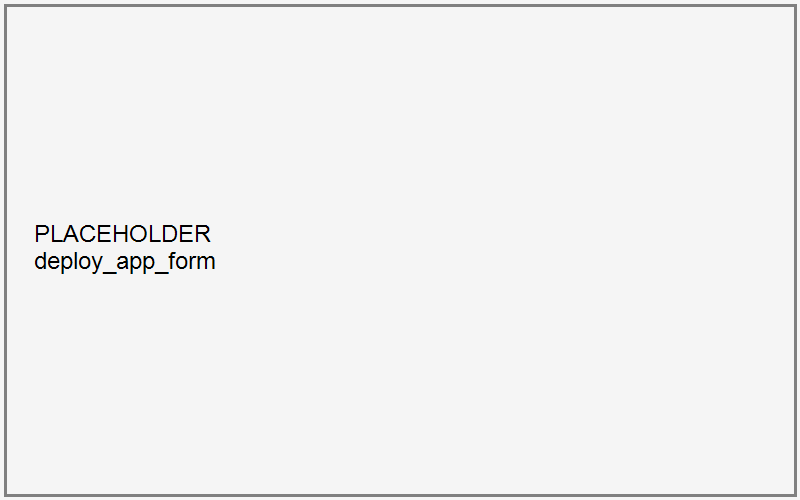
\includegraphics[width=13cm]{captures/deploy_app_form.png}
    \caption{Capture d'écran — Formulaire de déploiement d'une application}
    \label{fig:capture-deploy}
\end{figure}

\begin{figure}[h!]
 \centering
    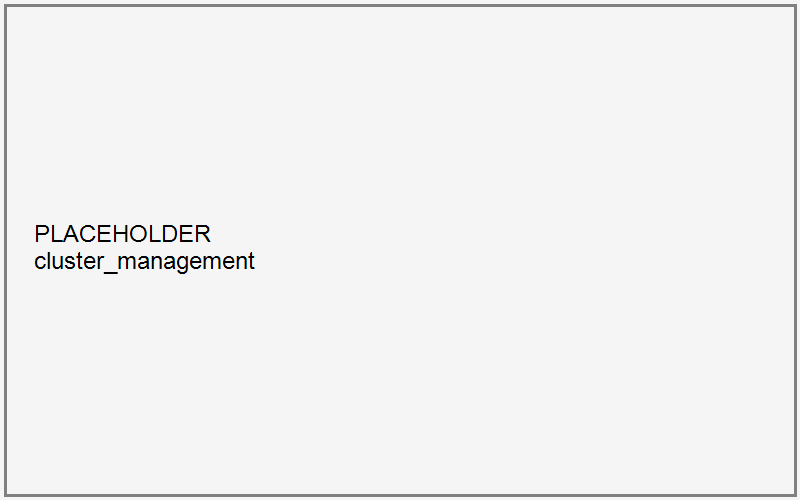
\includegraphics[width=13cm]{captures/cluster_management.png}
    \caption{Capture d'écran — Supervision du cluster (console d'administration)}
    \label{fig:capture-cluster}
\end{figure}

\subsection{Le pipeline CI/CD Frontend}

Deux pipelines Jenkins distincts (un pour le portail client, un pour la console d'administration) sont mis en place, reprenant le même squelette que le pipeline backend du Sprint 5 : construction (\texttt{npm run build}) produisant les fichiers statiques, construction de l'image de conteneur (Nginx servant ces fichiers statiques) via Kaniko, publication sur Docker Hub, puis mise à jour du déploiement Kubernetes correspondant.

\subsection{Difficultés rencontrées et solutions apportées}

\begin{itemize}
    \item \textbf{Duplication de code entre les deux applications React} : les deux applications partagent une quinzaine de fichiers quasi identiques (contexte d'authentification, client API, thème, composants de mise en page) sans outillage de monorepo ni paquet partagé. Cette duplication, assumée faute de temps disponible dans le sprint pour la refactoriser, est identifiée comme dette technique et reprise dans les limites du chapitre de validation.
    \item \textbf{Pipelines frontend moins robustes que le pipeline backend} : les pipelines du portail client et de la console d'administration ne reprennent pas l'ensemble des mécanismes de fiabilisation mis en place pour le pipeline backend au Sprint 5 (options anti-corruption de Kaniko, redémarrage systématique de Jenkins). \textit{Solution partielle} : ce point est traité au Sprint 10, consacré à l'optimisation du pipeline CI/CD.
\end{itemize}

\subsection{Résultat obtenu}

Au terme de ce sprint, les fonctionnalités principales de déploiement et de supervision d'applications, développées côté backend depuis la Release 1, sont accessibles au travers d'interfaces graphiques fonctionnelles, construites et déployées automatiquement.

\subsection{Conclusion du Sprint}

Ce sprint a rendu la plateforme utilisable de bout en bout par un utilisateur final pour son cas d'usage principal. Le sprint suivant complète l'interface graphique par les fonctionnalités restantes (Kafka, Eventing, facturation, équipe, audit).


\section{Sprint 9 : Finalisation du Frontend}

\subsection{Introduction}

Ce sprint a pour objectif de compléter l'interface graphique des deux applications avec l'ensemble des fonctionnalités développées côté backend lors des Releases 1 et 2, mais non encore exposées graphiquement à l'issue du Sprint 8.

\subsection{Objectifs du Sprint}

\begin{itemize}
    \item Développer les pages de gestion Kafka et de configuration de l'Eventing sur le portail client.
    \item Développer les pages de facturation, de gestion d'équipe et de paramètres du compte sur le portail client.
    \item Développer les pages de facturation globale, de journal d'audit et de gestion des utilisateurs sur la console d'administration.
    \item Mettre en place une page de statut public de la plateforme.
\end{itemize}

\subsection{Sprint Backlog}

\begin{table}[!ht]
\begin{center}
     \begin{tabular}{|l{11cm}|l{3cm}|}
     \hline
     \textbf{User Story} & \textbf{Statut} \\
     \hline
     En tant que client, je veux gérer mes sujets Kafka depuis le portail & Réalisé \\
     \hline
     En tant que client, je veux configurer des déclencheurs d'événement depuis le portail & Réalisé \\
     \hline
     En tant que client, je veux consulter ma facturation et gérer mon équipe & Réalisé \\
     \hline
     En tant qu'exploitant, je veux consulter le journal d'audit et la facturation globale & Réalisé \\
     \hline
     \end{tabular}
     \caption{Sprint Backlog — Sprint 9}
     \label{tab:sb-sprint9}
     \end{center}
\end{table}

\subsection{Présentation des composants développés}

\paragraph{Portail client.} Ajout des pages \texttt{KafkaTopics} et \texttt{Eventing} (gestion visuelle des sujets et des déclencheurs, cf. Sprint 6), \texttt{LogsView} et \texttt{Monitoring} (visualisation détaillée des journaux et métriques, cf. Sprint 7), \texttt{Billing} (facturation du compte, cf. modèle de facturation présenté au chapitre de modélisation), \texttt{Team} (gestion des membres et de leurs permissions, cf. Sprint 4), \texttt{Settings} et \texttt{StatusPage} (page de statut public de la plateforme).

\paragraph{Console d'administration.} Ajout des pages \texttt{AdminUsers} (gestion des utilisateurs), \texttt{AdminBilling} (facturation globale de la plateforme) et \texttt{AdminAuditLog} (journal d'audit des actions administratives, avec export).

\subsection{Présentation de la réalisation}

La figure~\ref{fig:capture-kafka} illustre la page de gestion des sujets Kafka du portail client, et la figure~\ref{fig:capture-billing} la page de facturation.

\begin{figure}[h!]
 \centering
    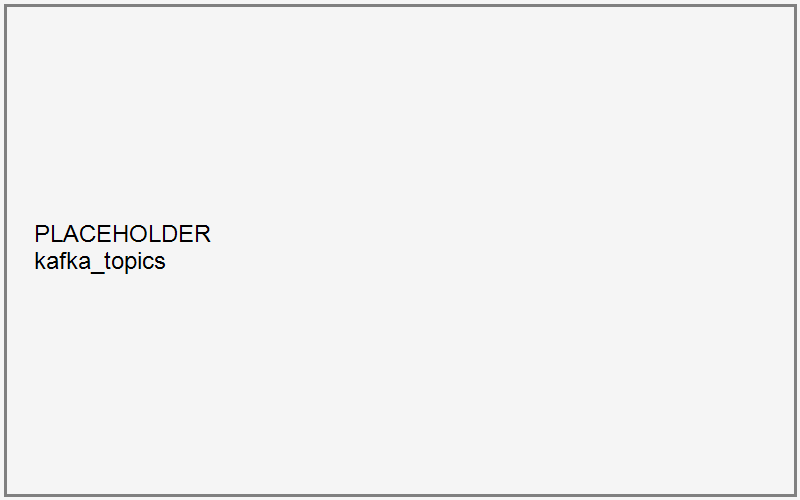
\includegraphics[width=13cm]{captures/kafka_topics.png}
    \caption{Capture d'écran — Gestion des sujets Kafka (portail client)}
    \label{fig:capture-kafka}
\end{figure}

\begin{figure}[h!]
 \centering
    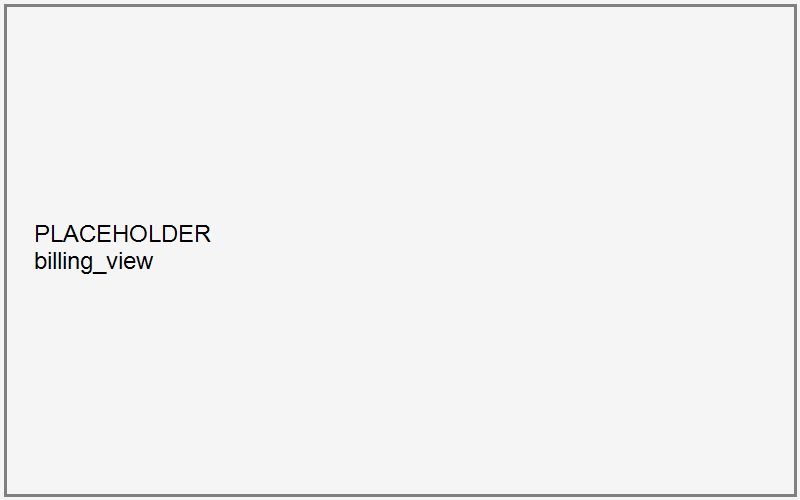
\includegraphics[width=13cm]{captures/billing_view.png}
    \caption{Capture d'écran — Facturation du compte client}
    \label{fig:capture-billing}
\end{figure}

\subsection{Difficultés rencontrées et solutions apportées}

\begin{itemize}
    \item \textbf{Simplification du périmètre de la console d'administration} : deux pages initialement prévues sur la console d'administration, dédiées à la gestion des incidents et à la détection d'anomalies (\texttt{AdminIncidents}, \texttt{AdminAnomalies}), ont finalement été retirées du menu de navigation afin de simplifier l'interface, la valeur ajoutée de ces vues étant jugée insuffisante par rapport à leur coût de maintenance à ce stade du projet. Il s'agit d'une décision de réduction de périmètre assumée, et non d'un abandon lié à une difficulté technique.
    \item \textbf{Décalage entre nom d'utilisateur et identifiant effectif dans les journaux affichés côté frontend} : une régression, apparue après la correction de l'isolation des journaux au Sprint 5, a conduit le frontend à transmettre le nom d'utilisateur plutôt que l'identifiant effectif attendu par le backend. \textit{Solution} : correction du frontend pour utiliser systématiquement l'identifiant effectif fourni par le contexte d'authentification.
\end{itemize}

\subsection{Résultat obtenu}

Au terme de ce sprint, l'ensemble des fonctionnalités backend développées depuis la Release 1 sont exposées et exploitables au travers des deux interfaces graphiques de la plateforme.

\subsection{Conclusion du Sprint}

Ce sprint achève le périmètre fonctionnel de l'interface utilisateur de la plateforme. Le sprint suivant se concentre sur l'industrialisation des chaînes d'intégration continue de l'ensemble des composants.


\section{Sprint 10 : Optimisation du pipeline CI/CD}

\subsection{Introduction}

Ce sprint a pour objectif de consolider et d'harmoniser les pipelines d'intégration continue des quatre composants de la plateforme (backend, portail client, console d'administration, et un pipeline distinct pour les microservices), en généralisant les mécanismes de fiabilisation mis au point empiriquement lors du Sprint 5 pour le pipeline backend.

\subsection{Objectifs du Sprint}

\begin{itemize}
    \item Harmoniser les quatre pipelines Jenkins existants sur un socle commun plus robuste.
    \item Fiabiliser l'exécution de Kaniko afin d'éviter les échecs de construction dus à la corruption de l'environnement Jenkins identifiée au Sprint 5.
    \item Clarifier l'usage des différents fichiers Dockerfile du backend, source de confusion identifiée lors de l'audit du projet.
\end{itemize}

\subsection{Sprint Backlog}

\begin{table}[!ht]
\begin{center}
     \begin{tabular}{|l{11cm}|l{3cm}|}
     \hline
     \textbf{User Story} & \textbf{Statut} \\
     \hline
     En tant qu'exploitant, je veux que les échecs de checkout Git soient automatiquement réessayés & Réalisé (backend uniquement) \\
     \hline
     En tant qu'exploitant, je veux que Kaniko ne corrompe plus l'environnement Jenkins & Réalisé (backend uniquement) \\
     \hline
     En tant qu'exploitant, je veux un pipeline unique et cohérent pour tous les composants & Non réalisé \\
     \hline
     En tant qu'exploitant, je veux une étape de tests automatisés dans les pipelines & Non réalisé \\
     \hline
     En tant qu'exploitant, je veux une analyse de sécurité des images construites & Non réalisé \\
     \hline
     \end{tabular}
     \caption{Sprint Backlog — Sprint 10}
     \label{tab:sb-sprint10}
     \end{center}
\end{table}

\subsection{Réalisation}

Les correctifs de fiabilisation identifiés au Sprint 5 (options Kaniko \texttt{--use-new-run}/\texttt{--snapshot-mode=redo}, redémarrage sécurisé systématique de Jenkins, réessai automatique du \textit{checkout} Git) demeurent, à l'issue de ce sprint, appliqués uniquement au pipeline du backend, qui reste le plus mature des quatre. Le remplacement du fichier \texttt{backend.Dockerfile} (construction multi-étapes avec utilisateur non privilégié, non utilisé en pratique par le pipeline) au profit exclusif de \texttt{backend-kaniko.Dockerfile} (construction mono-étape effectivement utilisée) a été clarifié dans la documentation technique du projet, sans toutefois que le premier fichier, devenu du code mort, n'ait été supprimé du dépôt.

\subsection{Difficultés rencontrées et limites assumées}

En toute rigueur, ce sprint doit être présenté avec honnêteté au regard de son objectif initial : \textbf{l'optimisation du pipeline CI/CD n'a été que partiellement atteinte}. Les difficultés suivantes, documentées par les audits menés sur la plateforme, n'ont pas été résolues dans le temps imparti du projet et sont reprises comme perspectives d'amélioration au chapitre de validation :

\begin{itemize}
    \item Les pipelines du portail client et de la console d'administration n'ont \textbf{pas} été alignés sur les mécanismes de fiabilisation du pipeline backend.
    \item Le pipeline dédié aux microservices reste le moins abouti des quatre : construction et publication d'image Docker classiques (sans Kaniko), absence d'identifiants explicites pour le \textit{checkout} Git, et absence de toute étape de déploiement Kubernetes final.
    \item Aucun des quatre pipelines ne comporte d'étape de tests automatisés (la compilation backend est réalisée avec l'option \texttt{-DskipTests}), d'analyse statique de code, ni d'analyse de vulnérabilités des images construites.
    \item Aucun mécanisme de \textit{rollback} automatique n'est déclenché en cas d'échec de la vérification du déploiement (\texttt{kubectl rollout status}).
\end{itemize}

Ces limites ne remettent pas en cause le fonctionnement de la plateforme, qui reste opérationnelle et déployée automatiquement à chaque évolution ; elles constituent en revanche des axes d'industrialisation identifiés mais non traités, dans un contexte de projet à ressources et délai contraints, où la priorité a été donnée à la robustesse fonctionnelle de la plateforme elle-même plutôt qu'à l'homogénéisation complète de ses quatre pipelines.

\subsection{Résultat obtenu}

Au terme de ce sprint, le pipeline backend demeure le plus robuste et le plus représentatif de la démarche CI/CD visée pour la plateforme ; les trois autres pipelines restent fonctionnels mais perfectibles, les limites identifiées étant explicitement documentées plutôt que dissimulées.

\subsection{Conclusion du Sprint}

Ce sprint clôt la Release 3. L'ensemble des composants de la plateforme (backend, deux frontends) sont désormais construits et déployés automatiquement, avec un niveau de maturité inégal selon le composant, honnêtement documenté. La Release suivante, consacrée à la validation, revient en détail sur l'ensemble de ces limites ainsi que sur les tests réalisés sur la plateforme dans son ensemble.

\section{Conclusion}

La Release 3 a rendu la plateforme pleinement utilisable par ses utilisateurs finaux, au travers de deux interfaces graphiques couvrant l'intégralité du périmètre fonctionnel développé depuis la Release 1, et a engagé un travail d'industrialisation des chaînes de déploiement continu. Ce travail d'industrialisation, présenté ici avec la même rigueur que les fonctionnalités abouties, n'a été que partiellement mené à son terme : ce constat, assumé, alimente directement le chapitre de validation qui clôt ce mémoire.
